\documentclass[aspectratio=169]{beamer}
%\usetheme{CambridgeUS}
%\usecolortheme{beaver}

%\usefonttheme{serif}
%\usepackage{helvet}

\usefonttheme{serif}     % Font theme: serif
%\usepackage{ccfonts}     % Font family: Concrete Math
\usepackage[T1]{fontenc} % Font encoding: T1

\setbeamersize{text margin left=42pt,text margin right=42pt} 
\setbeamertemplate{navigation symbols}{}
\setbeamertemplate{itemize items}[default]

\beamertemplatenavigationsymbolsempty

\definecolor{fore}{RGB}{51,51,51}
\definecolor{back}{RGB}{255, 254, 250}
\definecolor{title}{RGB}{ 255, 15, 0}
\definecolor{links}{RGB}{18, 168, 255}

\setbeamercolor{titlelike}{fg=title}
\setbeamercolor{normal text}{fg=fore,bg=back}
\setbeamercolor{alerted text}{fg=title}
\setbeamercolor{itemize item}{fg=title}
\setbeamercolor{enumerate item}{fg=title}
\hypersetup{colorlinks,urlcolor=links}

% for code https://kbroman.org/blog/2013/10/07/better-looking-latexbeamer-slides/
\usepackage{listings}
\definecolor{keywords}{RGB}{255,0,90}
\definecolor{comments}{RGB}{60,179,113}
\lstset{language=Python,
keywordstyle=color{keywords},
commentstyle=color{comments}emph}

% fonts
\usepackage[sc]{mathpazo}


% title info
\title{\textbf{Course Introduction}}
\subtitle{\textbf{GGR424 - Transportation Geography \& Planning}}
\author{Jeff Allen}
\institute{University of Toronto}
\date{January 10, 2022}


\begin{document}
	
\begin{frame}
	\titlepage	
\end{frame}



\begin{frame}
\textbf{Today:}
\begin{itemize}
	\item Introductions
	\item What is this course about?
	\item Course Outline
	\item Mode prioritization
	\item Class census
\end{itemize}
\end{frame}




\begin{frame}
\LARGE{\textbf{Introductions:}}
\end{frame}



\begin{frame}
\textbf{About Me}
\begin{itemize}
	\item PhD Candidate in Geography
	\item Researches Urban Geography/Planning, Transportation, \& GIS
	\item Cartographer / GIS
\end{itemize}
\end{frame}








\begin{frame}
	\textbf{What is this course about?}
	\begin{itemize}
		\item Beep
		\item Boop
	\end{itemize}
\end{frame}




%\begin{frame}
%\begin{columns}
%	\begin{column}{0.5\textwidth}
%		
%		\textbf{Passively contributed "Big" data} \\
%		\vspace{3mm}
%		\begin{itemize}
%			\item Big data - "data that can't fit into an Excel spreadsheet"
%			\item Collection via GPS, sensors, app usage, etc.
%			\item Often by large tech companies
%			\item e.g. Google Maps, Uber, Twitter, Visa, etc.
%		\end{itemize} 
%	\end{column}
%	
%	\begin{column}{0.5\textwidth}
%		\begin{figure}
%			\centering
%			\includegraphics[width=1\linewidth]{images/uber_surge.png}
%		\end{figure}
%		\tiny Source: \url{https://www.blogto.com/tech/2019/12/uber-lyft-surge-pricing-ttc-chaos-toronto/}
%	\end{column}
%	
%	
%	
%\end{columns}
%\end{frame}


%\begin{frame}
%	\textbf{Passively contributed "Big" data} - e.g. NY Times investigation into the smartphone tracking industry
%	\begin{figure}
%		\centering
%		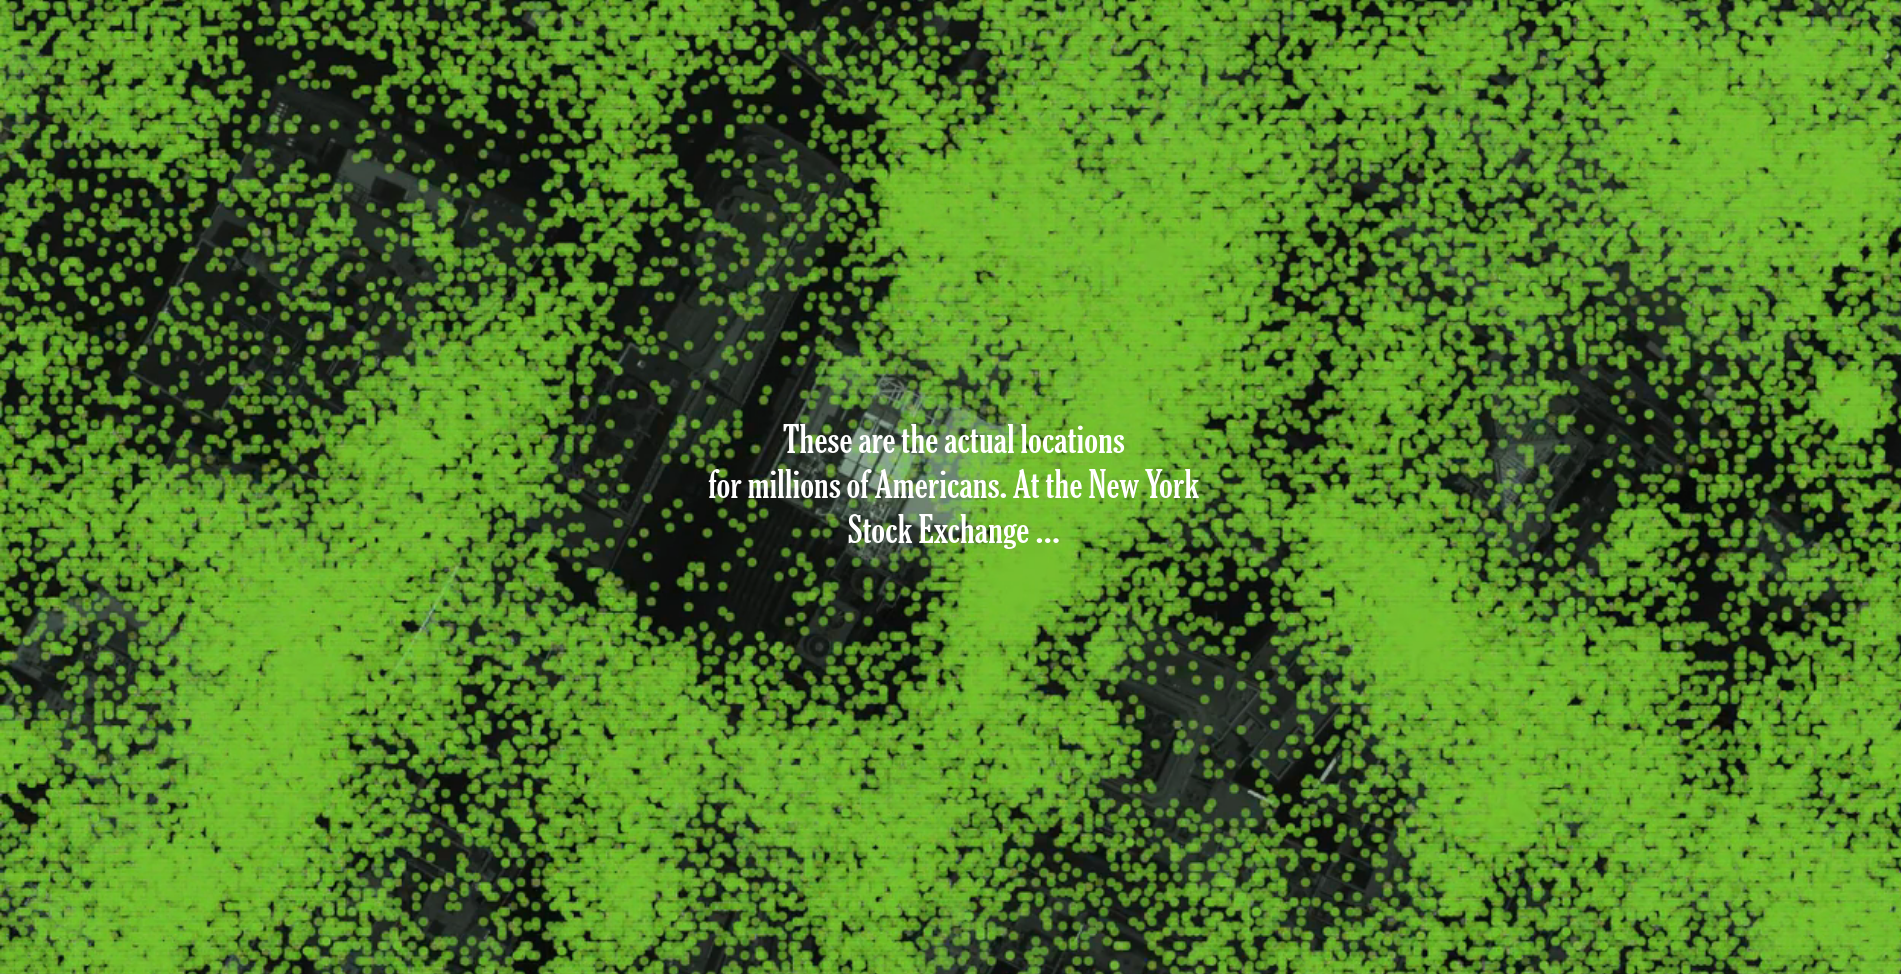
\includegraphics[width=0.8\linewidth]{images/nytimes_gps_stockexchange.png}
%	\end{figure}
%	\tiny\url{https://www.nytimes.com/interactive/2019/12/19/opinion/location-tracking-cell-phone.html}
%\end{frame}
%
%
%
%\begin{frame}
%Examples: \textbf{COVID Alert}
%\begin{figure}
%	\centering
%	\includegraphics[width=1\linewidth]{images/covid_alert.png}
%\end{figure}
%\tiny\url{https://www.canada.ca/en/public-health/services/diseases/coronavirus-disease-covid-19/covid-alert.html}
%\end{frame}



\begin{frame}
	\LARGE{\textbf{Course Outline \& Details:}}
\end{frame}









\begin{frame}
	\textbf{Next Week}
	
	\begin{itemize}
		\item Overview and history of geographic data sources
		\item Common structures and formats of geographic data
		\item Intro to QGIS 
		\item Overview of Assignment 1 (currently posted, due Sept 29)
	\end{itemize}

\end{frame}



\end{document}